\documentclass[fr]{../../../../../../eplexam}

\usepackage{../../../math-FSAB1103-exam}
\usepackage{../../../../../../eplunits}

\hypertitle{Math\'ematique}{3}{FSAB}{1103}{2015}{Janvier}
{Simon Demaré}
{Jean-François Remacle et Grégoire Winckelmans}

\section{(30$\%$)}
On considère l'EDP suivante pour $u(x,t)$ :
\begin{align*}
  \fpart{}{x}(cu) + \fpart{u}{t} &= S
\end{align*}
On a que $c=c(x) = c_0 \cos{(2 \pi \frac{x}{L})}$ avec $c_0$ et $L$ constants. La condition initiale est $u(s,0) = u_0 \cdot \exp(-\frac{s}{L_0})$ pour $s\geq 0$ avec $u_0$ une constante de même dimension que $u$ et $L_0$ une constante de longueur. La condition limite est $u(0, \tau) = u_0$ pour $\tau \geq 0$.

\begin{enumerate}
  \item
    Obtenez le réseau des caractéristiques  : équation pour la ``région A'' du quart de plan (i.e. relation entre $x$, $t$ et $s$) et équation  pour la ``région B'' du quart de plan (i.e. relation entre $x$, $t$ et $\tau$). Veuillez à finalement aussi exprimer explicitement $s$ en fonction de $x$ et $t$ (région A) et $\tau$ en fonction de $x$ et $t$ (région B).
  \item
    Faites un esquisse de $\frac{c(x)}{c_0}$. Faites ensuite une esquisse du réseau des caractéristiques (une esquisse propre, avec des axes adimensionnels et chiffrés !) en particulier esquissez celles qui émanent de $\frac{s}{L}=0,\frac{1}{4},\frac{1}{2},\frac{3}{4} \textrm{ et } 1$ et de $\frac{c_0 \tau}{L} = 0, \frac{1}{2}, 1$.
  \item
    Considérez le cas avec $S=0$.
    \begin{itemize}
      \item Obtenez la solution $u(x,t)$ dans la région A.
      \item Obtenez la solution $u(x,t)$ dans la région B.
      \item L'intégrale $I(t) = \int^{\infty}_0 u(x,t) dx$ est elle conservée au cours du temps et pourquoi ?
  \end{itemize}
  \item
    Considérez le cas avec $S=\frac{cu}{L}$
    \begin{itemize}
      \item Obtenez la solution $u(x,t)$ dans la région A.
      \item Obtenez la solution $u(x,t)$ dans la région B.
    \end{itemize}
\end{enumerate}

\subsection*{Aide}
\begin{align*}
\int \cos{(a \eta)} d\eta &= \dfrac{1}{a} \sin{(a\eta)}\\
\int \dfrac{d\eta}{\cos{(a \eta)}} &= \dfrac{1}{a} \cdot \ln\Big|\tan\Big(\dfrac{a \eta}{2} + \dfrac{\pi}{4}\Big)\Big|.
\end{align*}


\begin{solution}
  On réécrit l'EDP comme suit
  \begin{align*}
    c\fpart{u}{x} + \fpart{u}{t} &= -u\fpart{c}{x} + S
  \end{align*}
  \begin{enumerate}
    \item
      On a
      \begin{align*}
        \dif t & = \frac{\dif x}{c_0 \cos\left(2 \pi \frac{x}{L}\right)}
      \end{align*}
      \begin{description}
        \item[Région A]
          On intègre de $(s,0)$ à $(x,t)$:
          \begin{align*}
            \int_0^t \dif t & = \int_s^x \frac{\dif x}{c_0 \ln\left(2 \pi \frac{x}{L}\right)}\\
            t & = \frac{L}{2 \pi c_0}\left(\ln\Big|\tan\Big(\pi \frac{x}{L} + \frac{\pi}{4}\Big)\Big|-\ln\Big|\tan\Big(\pi \frac{s}{L} + \frac{\pi}{4}\Big)\Big|\right)\\
            \exp\Big(\frac{2 \pi tc_0}{L}\Big) & = \frac{\tan\Big(\pi \frac{x}{L} + \frac{\pi}{4}\Big)}{\tan\Big(\pi \frac{s}{L} + \frac{\pi}{4}\Big)}\\
            \tan\Big(\pi \frac{s}{L} + \frac{\pi}{4}\Big) & = \exp\Big(\frac{-2 \pi tc_0}{L}\Big)\tan\Big(\pi \frac{x}{L} + \frac{\pi}{4}\Big)
          \end{align*}
          Ici on ne peut pas juste passer à l'arctan car tan est périodique.
          Supposons qu'on parte de $s \in [k\pi;(k+1)\pi]$,
          on voit que $x$ part de $s$ en $t = 0$ et ne sait pas sortir de $[k\pi;(k+1)\pi]$ sinon la tan est infinie dans l'équation ci-dessus.
          Soit $k$ tel que $x \in [k\pi;(k+1)\pi]$, on a donc
          \begin{align*}
            s & = k\pi + \frac{L}{\pi}\arctan\left(\exp\Big(\frac{-2 \pi tc_0}{L}\Big)\tan\Big(\pi \frac{x}{L} + \frac{\pi}{4}\Big)\right) - \frac{L}{4}.
          \end{align*}
          Remarque que $s \to \infty$ lorsque $x \to \infty$, on en aura besoin plus tard.
        \item[Région B]
          On intègre de $(0,\tau)$ à $(x,t)$:
          \begin{align*}
            \int_\tau^t \dif t & = \int_0^x \frac{\dif x}{c_0 \ln\left(2 \pi \frac{x}{L}\right)}\\
            t-\tau & = \frac{L}{2 \pi c_0}\left(\ln\Big|\tan\Big(\pi \frac{x}{L} + \frac{\pi}{4}\Big)\Big|-\ln\Big|\tan\Big(\pi \frac{0}{L} + \frac{\pi}{4}\Big)\Big|\right)\\
            \tau & = t - \frac{L}{2 \pi c_0}\ln\Big|\tan\Big(\pi \frac{x}{L} + \frac{\pi}{4}\Big)\Big|\\
            \tau & = t - \frac{L}{2 \pi c_0}\ln\Big|\tan\Big(\pi \frac{x}{L} + \frac{\pi}{4}\Big)\Big|\\
          \end{align*}
      \end{description}
    \item
%     Le réseau des caractéristique est assez difficile à obtenir si on part de l'équation finale.
%
%     Pour le dessiner, faites l'esquisse de $c(x)/c_0$.
%     Ensuite, en chaque point $(x,t)$, dessinez la pente $(c(x),1)$.
%     Remarquez que la pente ne dépend pas de $t$ donc elle est la même sur tout l'axe vertical.
%     Ensuite essayez de faire des courbes qui sont tangentes à la pente que vous avez dessiner en chaque point.
    \item
      Pour la région A:
      \begin{align*}
        c_0 \frac{2\pi}{L} \sin\left(2\pi\frac{x}{L}\right) u \dif x & = c_0 \cos\left(2\pi\frac{x}{L}\right) \dif u\\
        \frac{2\pi}{L} \tan\left(2\pi\frac{x}{L}\right) \dif x & = \frac{1}{u} \dif u\\
        \int_s^x \frac{2\pi}{L} \tan\left(2\pi\frac{x'}{L}\right) \dif x' & = \int_{u(s,0)}^{u(x,t)} \frac{1}{u'} \dif u'\\
        \ln\cos\left(2\pi\frac{s}{L}\right) - \ln\cos\left(2\pi\frac{x}{L}\right) & = \ln u(x,t) - \ln u_0 + \frac{s}{L_0}\\
        u_0\exp \left(-\frac{s}{L_0}\right)\frac{\cos\left(2\pi\frac{s}{L}\right)}{\cos\left(2\pi\frac{x}{L}\right)} & = u(x,t)\\
      \end{align*}
      et il faut injecter $s$ maintentant, faites le.

      Pour la région B:
      \begin{align*}
        \int_0^x \frac{2\pi}{L} \tan\left(2\pi\frac{x'}{L}\right) \dif x' & = \int_{u(0,\tau)}^{u(x,t)} \frac{1}{u'} \dif u'\\
        \ln\cos(0) - \ln\cos\left(2\pi\frac{x}{L}\right) & = \ln u(x,t) - \ln u_0\\
        \frac{u_0}{\cos\left(2\pi\frac{x}{L}\right)} & = u(x,t).
      \end{align*}

      On a
      \begin{align*}
        \fdif{I(t)}{t}
        & = \int_0^\infty \fpart{u(x,t)}{t} \dif x\\
        & = \int_0^\infty -\fpart{(c(x)u(x,t))}{x} \dif x\\
        & = -[c(x)u(x,t)]_0^\infty\\
        & = c(0)u(0,t) - \lim_{x \to \infty} c(x) u(x,t).
      \end{align*}
      Rappelons-nous que pour $x \to \infty$, on est dans la région A et $s \to \infty$,
      on voit donc avec notre solution que du coup $u(x,t) \to 0$.
      Pour $x = 0$, on est dans la région B. On a donc
      \begin{align*}
        \fdif{I(t)}{t} & = c_0u_0
      \end{align*}
      ce n'est pas 0, $I(t)$ n'est donc pas conservé au cours du temps.
    \item
      Pour la région A:
      \begin{align*}
        c_0 \frac{2\pi}{L} \sin\left(2\pi\frac{x}{L}\right) u(x,t) \dif x + \frac{c(x)u(x,t)}{L} \dif x & = c(x) \dif u\\
        \frac{2\pi}{L} \tan\left(2\pi\frac{x}{L}\right) \dif x + \frac{1}{L} \dif x & = \frac{1}{u} \dif u\\
        \int_s^x \frac{2\pi}{L} \tan\left(2\pi\frac{x'}{L}\right) + \frac{1}{L} \dif x' & = \int_{u(s,0)}^{u(x,t)} \frac{1}{u'} \dif u'\\
        \ln\cos\left(2\pi\frac{s}{L}\right) - \ln\cos\left(2\pi\frac{x}{L}\right) + \frac{x-s}{L} & = \ln u(x,t) - \ln u_0 + \frac{s}{L_0}\\
        u_0\exp \left(\frac{x-s}{L}-\frac{s}{L_0}\right)\frac{\cos\left(2\pi\frac{s}{L}\right)}{\cos\left(2\pi\frac{x}{L}\right)} & = u(x,t)\\
      \end{align*}
      et il faut injecter $s$ maintentant, faites le.

      Pour la région B:
      \begin{align*}
        \int_0^x \frac{2\pi}{L} \tan\left(2\pi\frac{x'}{L}\right) + \frac{1}{L} \dif x' & = \int_{u(0,\tau)}^{u(x,t)} \frac{1}{u'} \dif u'\\
        \ln\cos(0) - \ln\cos\left(2\pi\frac{x}{L}\right) + \frac{x}{L} & = \ln u(x,t) - \ln u_0\\
        u_0 \frac{\exp\left(\frac{x}{L}\right)}{\cos\left(2\pi\frac{x}{L}\right)} & = u(x,t).
      \end{align*}
  \end{enumerate}
\end{solution}

\clearpage

\section{(25$\%$)}
On considère l'EDP suivante pour $u(x,t)$
\begin{align*}
\alpha \dfrac{\partial^2 u}{\partial x^2} = \dfrac{\partial u}{\partial t}
\end{align*}
avec $\alpha > 0$ constant. Le domaine est borné : $0 \leq x \leq L$. La condition initiale est $u(x,0) = u_0 (1-\frac{x}{L})$ avec $u_0 > 0$ constant. Pour $t>0$, les conditions aux limites sont $\frac{\partial u}{\partial x}(0,t) = 2 \frac{u_0}{L}$ et $u(L,t) = u_0$.
\begin{enumerate}
\item
De quel type d'EDP s'agit il, physiquement et mathématiquement ? Qu'est ce que $\alpha$ ? Qu'est ce qu'un temps ``court'' pour le problème présent, $0 < t \ll ...$ ?
\item
Sans encore résoudre mathématiquement le problème, esquissez la graphe attendu de $\frac{u}{u_0}$ en fonction de $\frac{x}{L}$ en des temps différents : $t=0$ (CI), temps court, temps moyen, temps long, temps très long (solution de régime).
\item
Obtenez ensuite, mathématiquement, la solution $u(x,t)$ du problème :
\begin{itemize}
\item Obtenez d'abord la solution en régime.
\item Obtenez ensuite la solution transitoire, avec séparation des variables.
\end{itemize}
\end{enumerate}

\subsection*{Aide}
\begin{align*}
\int \eta \sin{(a \eta)} d\eta &= \dfrac{1}{a^2} \sin{(a \eta)} - \dfrac{1}{a} \cdot \eta \cos{(a \eta)}\\
\int \eta \cos{(a \eta)} d\eta &= \dfrac{1}{a^2} \cos{(a \eta)} + \dfrac{1}{a} \cdot \eta \sin{(a \eta)}
\end{align*}


\begin{solution}
  \begin{enumerate}
    \item
      Une EDP de diffusion, $\alpha$ est le coefficient de diffusivité.
      Ses unités sont \si{\meter\squared\per\second} donc $L^2/\alpha$ est en \si{\second}.
      Un temps court est un temps $t$ tel que $0 < t \ll L^2/\alpha$.
    \item On trouve la solution de u pour différents temps à la figure \ref{fig:diff}
    \begin{solfig}{diff}{Solution pour différents temps}
	    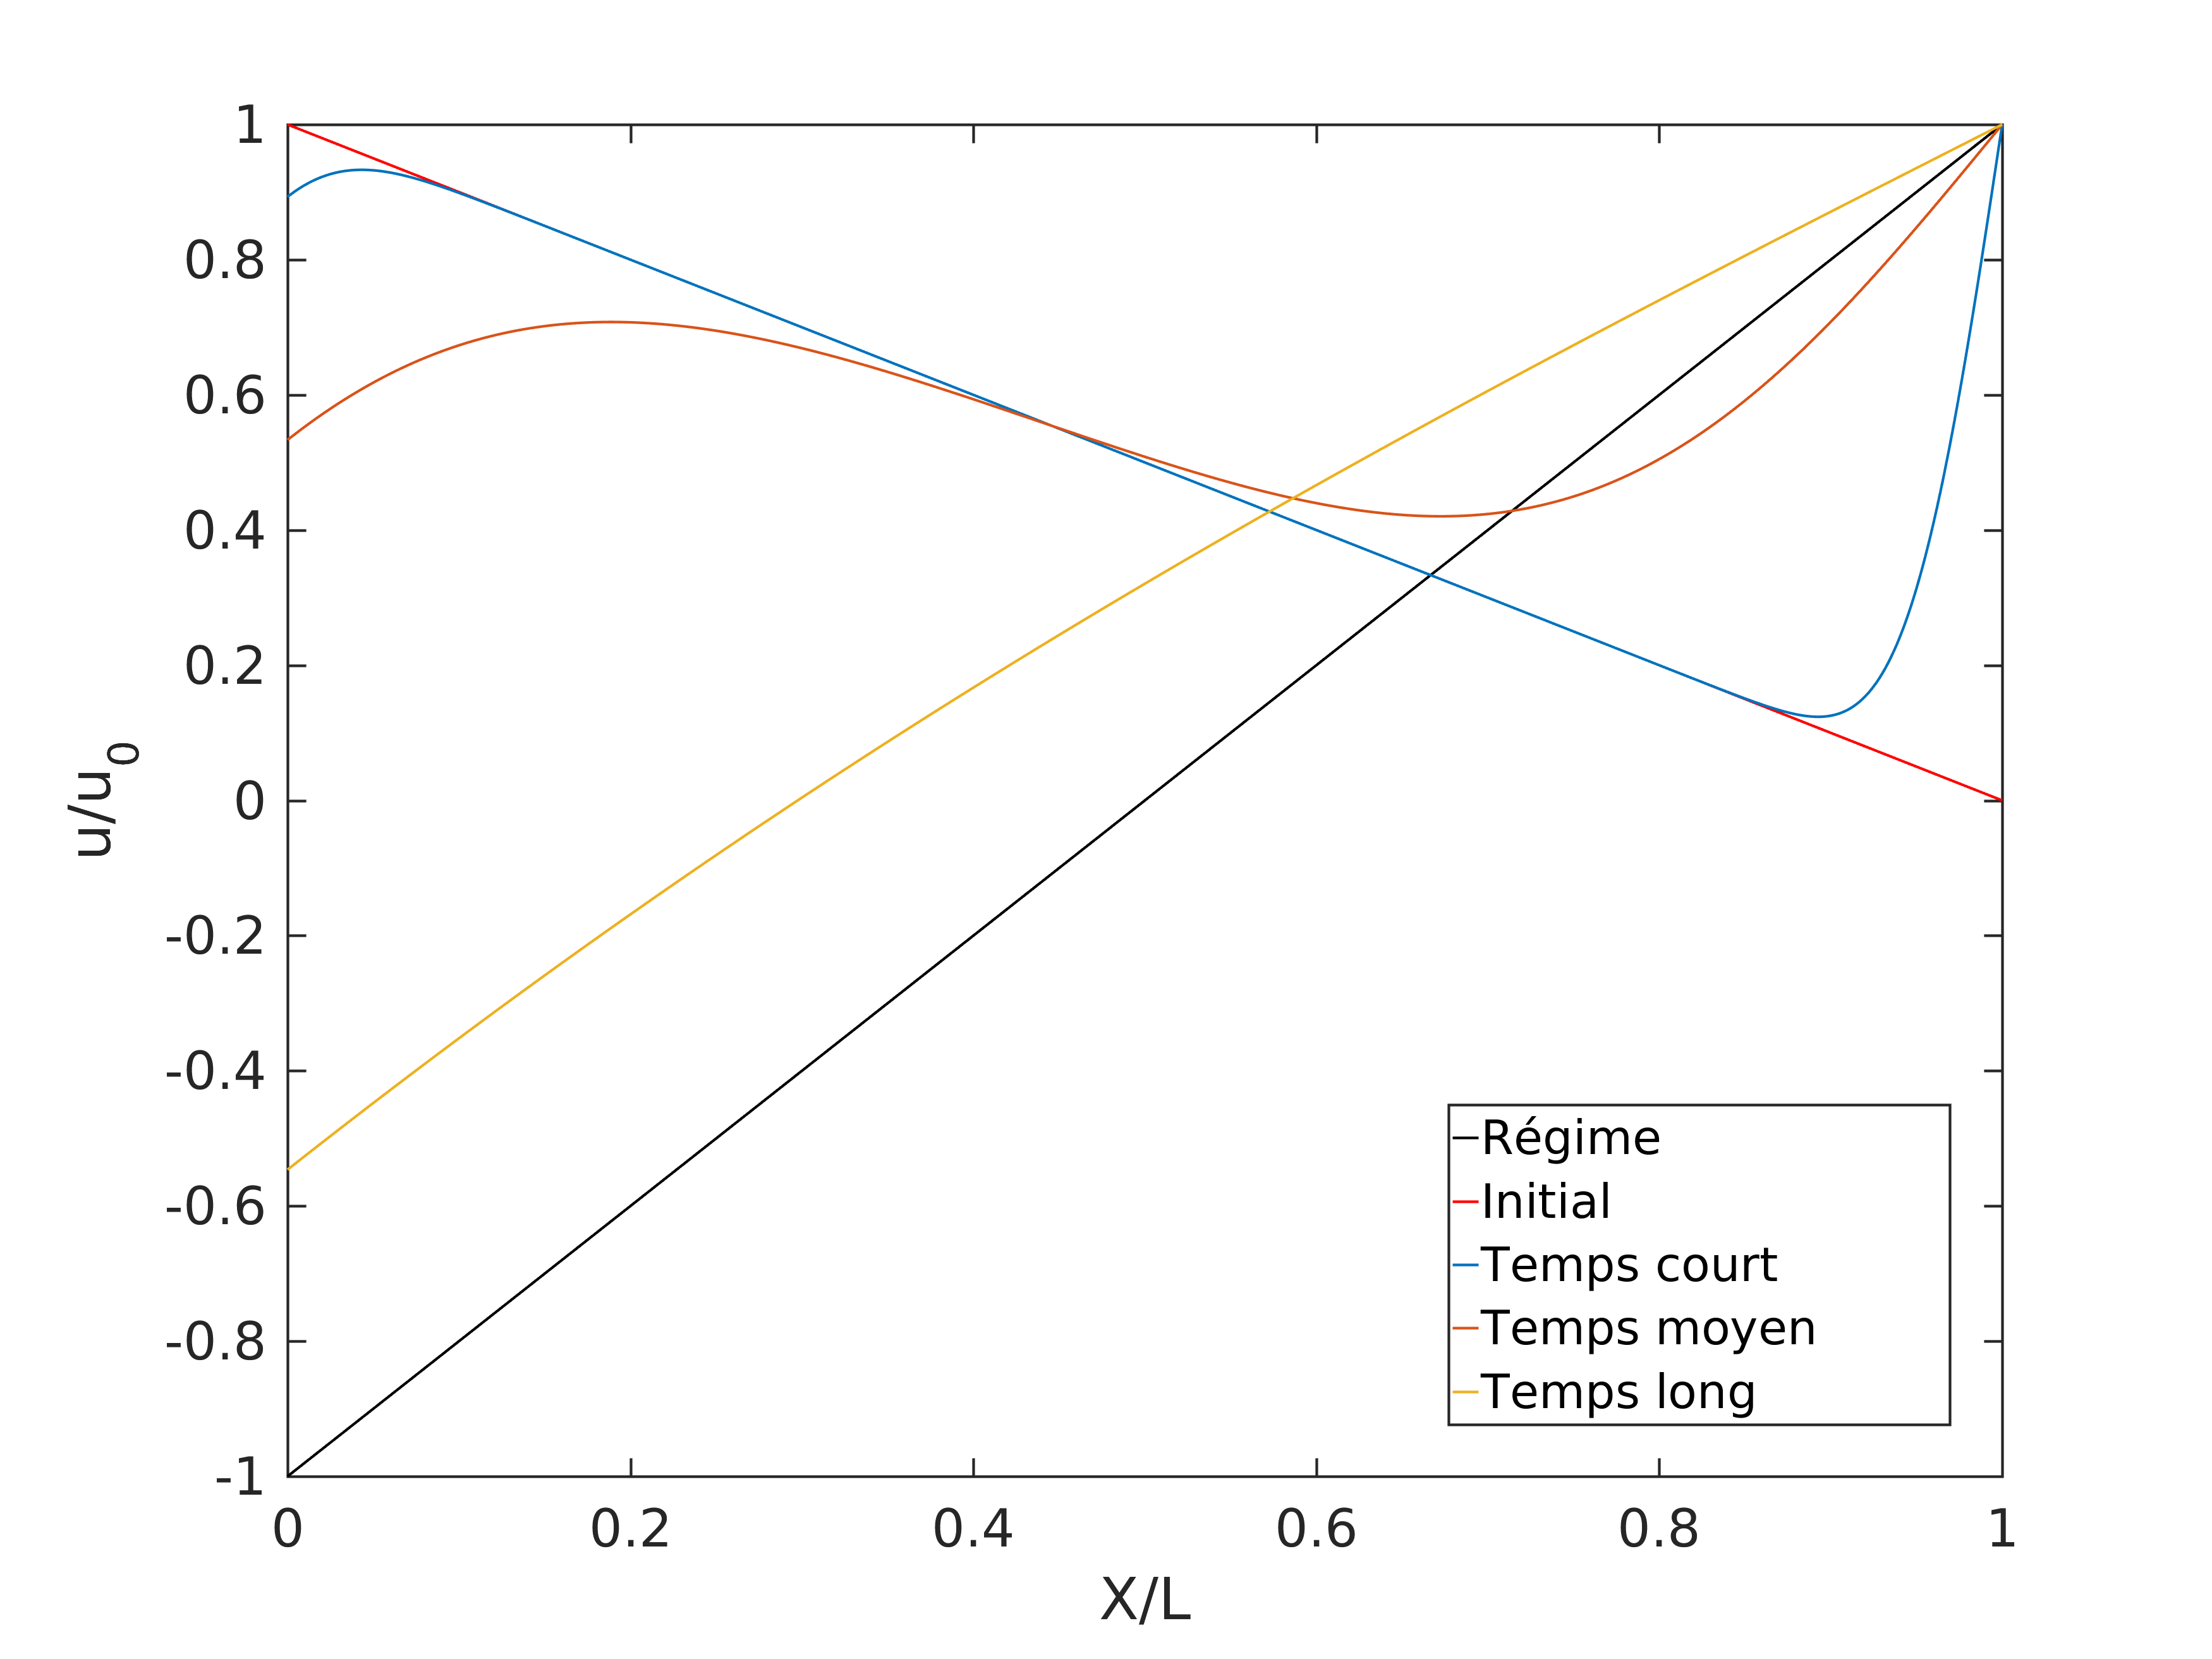
\includegraphics[width=0.8\textwidth]{diff.png}
    \end{solfig}
    \item
      On a
      \[ \frac{T'}{\alpha T} = \frac{X''}{X} = \pm k^2 \]
      On distingue 3 cas
      \begin{itemize}
        \item Si $k \neq 0$ et qu'on prend $+k^2$, $T_+(t) = C_+\exp(\alpha k^2t)$.
          Comme $\alpha > 0$, c'est une exponentielle croissante qui tend vers l'infini en $t \to \infty$.
          C'est vraiment une solution transitoire ça, on rejette.
        \item Si $k \neq 0$ et qu'on prend $-k^2$, $T = C\exp(-\alpha k^2t)$.
          Comme $\alpha > 0$, ça tend vers 0 lorsque $t \to \infty$, ça c'est une solution transitoire.
          On a également $X(x) = A \cos(kx) + B \sin(kx)$.
          Comme les solutions aux frontières $x = 0$ et $x=L$ ne dépendent pas de $t$,
          on doit avoir $X'(0) = 0$ et $X(L) = 0$, ce sera la solution en régime qui ne sera pas 0 en $x = 0$ et $x = L$.
          On a donc
          \begin{align*}
            -A k\sin(k0) + B k \cos(k0) &= 0\\
            A \cos(kL) + B \sin(kL) &= 0
          \end{align*}
          La première équation implique que $B = 0$ et donc on doit avoir $A\cos(kL) = 0$.
          Si $A = 0$, on a la solution triviale.
          Si $A \neq 0$, on a $k_n = (2n-1) \frac{\pi}{2L}$.
          On a donc
          \[ u(x,t) = \sum_{n=0}^\infty A_n' \exp(-\alpha k_n^2t) \cos(k_nx). \]
        \item Si $k = 0$, on a $X(x) = A_0x + B_0$ et $T(t) = C_0$.
          Ce qui donne $u(x,t) = D_0' x + E_0'$.
          Comme la solution vaut 0 pour les conditions en $x = 0$ et $x = L$, on a
          $u(L,t) = u_0$ et $\fpart{u}{x}(0,t) = 2\frac{u_0}{L}$ donc $D_0' = 2\frac{u_0}{L}$ et $E_0' = -u_0$, c'est à dire
          \[ u(x,t) = 2\frac{u_0}{L} x - u_0. \]
      \end{itemize}
      Au total, on a
      \[ u(x,t) = R(x) + \Theta(x,t) = 2\frac{u_0}{L} x - u_0 + \sum_{n=0}^\infty A_n' \exp(-\alpha k_n^2t) \cos(k_nx). \]
      On doit maintenant s'assurer qu'on respecte la condition initiale en $t = 0$, c'est à dire
      \begin{align*}
        2\frac{u_0}{L} x - u_0 + \sum_{n=0}^\infty A_n' \cos(k_nx) & = u_0 - u_0\frac{x}{L}\\
        \sum_{n=0}^\infty A_n' \cos(k_nx) & = 2u_0 - 3u_0\frac{x}{L}.
      \end{align*}
      En multipliant par $\cos(k_mx)$ et intégrant de $0$ à $L$, on a
      \begin{align*}
        \frac{L}{2} A_m' & = u_0\int_0^L 2\cos(k_mx) - 3\frac{x}{L} \cos(k_m x) \dif x\\
        A_m'
        & = u_0 \frac{2}{L} \left[\frac{2}{k_m}\sin(k_mx) - \frac{3}{Lk_m^2} \cos(k_m x) - \frac{3}{k_m} \frac{x}{L} \sin(k_m x)\right]_0^L\\
        & = u_0 \frac{2}{L} \left(\frac{2}{k_m}\sin(k_mL) - \frac{3}{Lk_m^2} \cos(k_m L) - \frac{3}{k_m} \sin(k_m L) + \frac{3}{Lk_m^2}\right)\\
        & = u_0 \frac{2}{L} \left(\frac{2}{k_m}\sin((2m-1)\frac{\pi}{2}) - \frac{3}{k_m} \sin((2m-1)\frac{\pi}{2}) + \frac{3}{Lk_m^2}\right)\\
        & = u_0 \frac{2}{L} \left(-\frac{1}{k_m} \sin((2m-1)\frac{\pi}{2}) + \frac{3}{Lk_m^2}\right)\\
        & = u_0\frac{4}{(2m+1)\pi} \left(\frac{6}{(2m+1)\pi} + (-1)^{n}\right).
      \end{align*}
  \end{enumerate}
\end{solution}

\clearpage

\section{(25$\%$)}
On considère la fonction
\begin{align*}
w &= \arctan z\\
&= \dfrac{i}{2} \log{\dfrac{i+z}{i-z}}\\
&= \int^z_0 \dfrac{d\tilde{z}}{1+\tilde{z}^2} \dif \tilde{z} \quad \textrm{avec }z \neq \pm i
\end{align*}

\begin{enumerate}
\item
Montrez que la définition de $w$ est bien telle que $\tan w = z$.
\item
Obtenez le(s) point(s) de branchement. Utilisez aussi une esquisse et proposez un choix de coupure(s) qui soit compatible avec le fait de pouvoir évaluer $w$ pour $z$ purement réel. Définissez aussi la branche principale, $D_0$. Pour la suite on n'utilisera plus que celle-ci.
\item
Obtenez l'expression de $w$ pour le cas $z = iy$ avec $-1 \leq y < 1$. (Esquisse). A partir de ce résultat, obtenez aussi l'expression de $\arctanh(y)$
\item
Obtenez le développement en série de $w$ au tour de $z_0 = 0$. Quel est le rayon de convergence de cette série ? Pourquoi ?
\end{enumerate}

\subsection*{Aide}
\begin{align*}
\sin z &= \dfrac{1}{i} \sinh{(iz)} = \dfrac{1}{2i} (e^{iz}-e^{-iz})\\
\cos z &= \cosh{(iz)} = \dfrac{1}{2} (e^{iz}+e^{-iz})\\
\end{align*}
Pour $|Z| < 1$ on a aussi que $\dfrac{1}{1+Z} = 1-Z+Z^2-Z^3+...$ et que $\log{(1+Z)} = Z - \frac{1}{2} Z^2 + \frac{1}{3} Z^3$

\begin{solution}
  Voir Janvier 2013.
\end{solution}

\clearpage

\section{(20$\%$)}
Résoudre
\begin{equation*}
\int^{\infty}_0 \frac{x^p}{1+x^2} \dif x \quad \textrm{avec }0 < p < 1
\end{equation*}

Note:
Tous les formes des lemmes de Jordan étaient donnés.


\begin{solution}
  On a un pôle en $\pm i$ et un point de branchement en 0.
  Choisissons un contour en demi-cercle avec un encoche en 0 et un coupure de $[-\frac{\pi}{2}; \frac{3\pi}{2}]$ pour ne pas
  que notre coupure coupe notre demi-cercle encoché.

  On prouve à l'aide des lemmes de Jordans que l'intégrale sur l'encoche et sur le contour du demi-cercle tend vers 0.

  On a, en posant $y = -x$,
  \[ \int_{-\infty}^0 \frac{y^p}{1+y^2} \dif y = (-1)^p\int_0^\infty \frac{x^p}{1+x^2} \dif x \]
  Le résidu en $i$ vaut $-\frac{i^{p+1}}{2}$ et $-i$ n'est pas dans le contour.
  On a donc
  \[ (1 + (-1)^p)\int^{\infty}_0 \frac{x^p}{1+x^2} \dif x = -\frac{i^{p+1}}{2} 2\pi i = \pi i^p \]
  d'où

    $$(1 + \cos(p\pi) + i \sin(p\pi)) I =\pi i^{p}$$
par identification des parties réelles et imaginaires 
$$ I = \frac{\pi i^{p}}{1 + \cos(p \pi)}$$
\end{solution}
\end{document}
